%!TEX root = ED_Arvore.tex

\section{Árvore Binária}
\begin{frame}[label=notas]
	\begin{exampleblock}{Definição}
		Conjunto finito de elementos que está vazio ou  pode ser particionado em três subconjuntos disjuntos:
			\begin{itemize}
				\item Raiz, um subconjunto que possui um único elemento
				\item Subárvore esquerda, que é uma árvore binária
				\item Subárvore direita, também uma árvore binária
			\end{itemize}
	\end{exampleblock}

	\pause
	\begin{columns}
		\column{.15\textwidth}\centering
			\Tree [ .10 [ .5 ] ]
		\column{.1\textwidth}\centering
			\Tree [ .10
					[ .5 \edge[white]; [ .\node(n1){}; ]
						[ .8 ] ]
					\edge[white]; [ .\node(n2){}; ] ]
		\column{.15\textwidth}\centering
			\Tree [ .10
					\edge[white]; [ .\node(n1){}; ]
					[ .15
						[ .12 ]
						\edge[white]; [ .\node(n2){}; ] ] ]
		\column{.25\textwidth}\centering
			\Tree [ .10
					[ .5
						[ .1 ] [ .7 ] ]
					[ .14
						[ .12 ] [ .17 ] ] ]
		\column{.4\textwidth}\centering
			\Tree [ .10
					[ .5
						[ .3 [ .1 ] [ .4 ] ]
						[ .7 [ .8 ] ] ]
					[ .14
						[ .12  [ .11 ] [ .13 ] ]
						[ .17 ] ] ]
	\end{columns}
\end{frame}

\begin{frame}[label=notas]
	\framesubtitle{\subsecname\ (de Busca) \emph{vs} Árvores}

	\uncover<3->{
	\begin{exampleblock}{Árvore Binária de Busca}
		É uma árvore binária \alert<2>{ordenada}.
	\end{exampleblock}}
	\begin{itemize}
		\item \uncover<2->{Os nós de uma árvore binárias não podem ter mais de dois filhos, enquanto não há limites para o número de filhos de uma árvore}
		\item \uncover<4->{A árvore binária de busca tem os filhos ordenados segundo um certo critério}
	\end{itemize}
	\vspace{-.5\baselineskip}
	\uncover<4->{
	\begin{center}
		\LARGE
		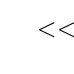
\begin{tikzpicture}[->]
			\Tree [ .50
				\edge node[auto=right]{{\small \alert{$<$}}}; [ .17
					\edge node[auto=right]{{\small \alert{$<$}}}; [ .12
						\edge node[auto=right]{{\small \alert{$<$}}}; [ .9 ]
						\edge node[auto=left]{{\small \alert{$<$}}}; [ .14 ] ]
					\edge node[auto=left]{{\small \alert{$<$}}}; [ .23
						\edge node[auto=right]{{\small \alert{$<$}}}; [ .19 ] \edge[white]; [ .\node(n1){}; ] ] ]
				\edge node[auto=left]{{\small \alert{$<$}}}; [ .72
					\edge node[auto=right]{{\small \alert{$<$}}}; [ .54 \edge[white]; [ .\node(n1){}; ]
					\edge node[auto=left]{{\small \alert{$<$}}}; [ .67 ] ]
					\edge node[auto=left]{{\small \alert{$<$}}}; [ .76 ] ] ]
		\end{tikzpicture}
	\end{center}
	}
\end{frame}

\subsection{Árvore Binária de Busca}
\begin{frame}[label=notas]
	\framesubtitle{Aplicações}

	\begin{itemize}
		\item Indexação em bancos de dados.
		\item Busca/ordenação em geral.
		\item Filas de prioridade
		\item Codificação de Huffman: método de compressão
			\subitem{Para atribuir aos caracteres mais freqüentes os códigos binários de menor comprimento, constrói-se uma árvore binária baseada nas probabilidades de ocorrência de cada símbolo.}
		\item Linguagens de programação:
			\begin{itemize}
				\item LISP - \textbf{cons}, \textbf{cdr}, etc.
				\item C++ - \textbf{set}, \textbf{map}, etc.
			\end{itemize}
		\item Representação de hierarquia (HTML, XML, etc.) - não necessariamente binárias
		\item etc.
	\end{itemize}
\end{frame}

\lstset{morekeywords={bt_dado_t}}%
\begin{frame}[fragile,label=notas]
	\framesubtitle{Implementação}

	\pause
	\begin{center}
		\begin{minipage}{.8\textwidth}
		\begin{lstlisting}[language=C,emph={esq},emphstyle=\color{blueUnB}\textbf,emph={[2]dir},emphstyle={[2]\color{greenUnB}\textbf}]
		/** Define o item da arvore. */
		typedef struct bt_item_t {
		    bt_dado_t dado;       	// O dado a ser armazenado.
		    struct bt_item_t *esq;	// Referencia para o filho a esquerda.
		    struct bt_item_t *dir;	// Referencia para o filho a direita.
		} bt_item_t;
		\end{lstlisting}
		\end{minipage}
		\vfill
		\begin{tikzpicture}[->,every node/.style={btnode}]
			\Tree [ .{\nodepart{two} 10}
					[ .{\nodepart{two} 5}
						[ .{\nodepart{two} 1} ]
						[ .{\nodepart{two} 8} ] ]
					[ .{\nodepart{two} 15}
						 \edge[white]; [ .\node[circle, draw=white](n1){}; ]
						[ .{\nodepart{two} 50}
							[ .{\nodepart{two} 16} ]
							[ .{\nodepart{two} 100} ] ] ] ]
		\end{tikzpicture}
	\end{center}
\end{frame}
\lstset{morekeywords={bt_item_t}}%

\begin{frame}[fragile,label=notas]
	\framesubtitle{Operações}

	\begin{columns}
		\column{.4\textwidth}
			\begin{itemize}
				\item criar
				\item esvaziar
				\item inserir
				\item remover
				\item buscar
				\item etc.
			\end{itemize}
		\column{.55\textwidth}
			\vfill\pause
			\begin{lstlisting}[title=Exemplo]
				bt_node_t * irmao(bt_node_t *node) {
				  if(!node->pai) return NULL;

				  if(node->pai->esq == node)
				    return node->pai->dir;
				  else
				    return node->pai->esq;
				}
			\end{lstlisting}
	\end{columns}
\end{frame}

% \begin{frame}[fragile,label=notas]
% 	\framesubtitle{Operações}

% 	\begin{center}
% 		\begin{minipage}{.55\textwidth}
% 			\begin{lstlisting}[language=C,title=Esvaziar,morekeywords={bt_item_t,bt_libera_dado,NULL}]
% 				void bt_esvazia(bt_item_t **ptr_raiz) {
% 				    if(!ptr_raiz || !(*ptr_raiz))
% 				        return;

% 				    bt_esvazia(&((*ptr_raiz)->esq));
% 				    bt_esvazia(&((*ptr_raiz)->dir));
% 				    bt_libera_dado(&((*ptr_raiz)->dado));
% 				    *ptr_raiz = NULL;
% 				}
% 			\end{lstlisting}
% 		\end{minipage}
% 	\end{center}
% \end{frame}

% \begin{frame}[fragile,label=notas]
% 	\framesubtitle{Operações}

% 	\begin{center}
% 		\begin{minipage}{.9\textwidth}
% 			\begin{lstlisting}[language=C,title=Busca,morekeywords={bt_item_t,bt_dado_t,NULL}]
% 				bt_item_t ** bst_busca(bt_item_t **ptr_raiz, bt_dado_t *dado) {
% 				    if(!ptr_raiz || !(*ptr_raiz))
% 				        return NULL;

% 				    if(dado < (*ptr_raiz)->dado)
% 				        return bst_busca(&((*ptr_raiz)->esq), dado);
% 				    if(dado > (*ptr_raiz)->dado)
% 				        return bst_busca(&((*ptr_raiz)->dir), dado);

% 				    return ptr_raiz;
% 				}
% 			\end{lstlisting}
% 		\end{minipage}
% 	\end{center}
% \end{frame}

% \begin{frame}[fragile,label=notas]
% 	\framesubtitle{Operações}

% 	\begin{center}
% 		\begin{minipage}{.9\textwidth}
% 			\begin{lstlisting}[title=Inserir]
% 				void bst_insere(bt_item_t **ptr_raiz, dado_t dado) {
% 				    if(!(*ptr_raiz))
% 				        *ptr_raiz = novo_bt_node(dado, NULL, NULL);
% 				    else if((*ptr_raiz)->dado > dado)
% 				        bst_insere(&(*ptr_raiz)->esq, dado);
% 				    else
% 				        bst_insere(&(*ptr_raiz)->dir, dado);
% 				}
% 			\end{lstlisting}
% 		\end{minipage}
% 	\end{center}
% \end{frame}

\begin{frame}[label=notas]
	\framesubtitle{Operação Remover}

	Remover é mais complicado... \pause O nó a ser removido pode ser
	\begin{columns}[T]
		\column{.3\textwidth}\centering
			\subitem{uma folha}
		\column{.3\textwidth}\centering
			\subitem{um galho}
		\column{.3\textwidth}\centering
			\subitem{uma raiz}
	\end{columns}
	\pause\vfill
	As situações existente são \emph{remover um nó com}:
	\begin{itemize}
		\item[0] filhos \pause - muito fácil
		\item[1] filho \pause - fácil
		\item[2] filhos \pause - complexo... pode ser feito por fusão ou cópia
	\end{itemize}
\end{frame}

\begin{frame}[label=notas]
	\framesubtitle{Operação Remover}

	Remoção de nó com 0 filhos:\pause
		\subitem{O nó é simplesmente retirado, e seu pai recebe nulo no lugar do ponteiro para aquele filho}

	\begin{columns}[T]
		\Large
		\column{.5\textwidth}\centering
			\begin{tikzpicture}[->]
				\Tree [ .C [ .A \node[red] {B}; ] [ .E [ .D ] [ .F ] ] ]
			\end{tikzpicture}
		\column{.5\textwidth}\centering
			\begin{tikzpicture}[->]
				\Tree [ .C [ .A ] [ .E [ .D ] [ .F ] ] ]
			\end{tikzpicture}
	\end{columns}
\end{frame}

\begin{frame}[label=notas]
	\framesubtitle{Operação Remover}

	Remoção de nó com 1 filho:\pause
		\subitem{O nó é retirado e em seu lugar toa a subárvore cuja raiz é seu
		filho toma o lugar; o pai do nó a ser retirado aponta para o filho do nó
		a ser retirado.}

	\begin{columns}[T]
		\Large
		\column{.5\textwidth}\centering
			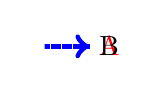
\begin{tikzpicture}[->]
				\Tree [ .C [ .\node[red] (a) {A}; [ .\node (b) {B}; ] ] [ .E [ .D ] [ .F ] ] ]
				\draw[dotted,blue,->, line width=2pt] (b)..controls +(west:1) and +(west:1) .. (a);
			\end{tikzpicture}
		\column{.5\textwidth}\centering
			\begin{tikzpicture}[->]
				\Tree [ .C [ .B ] [ .E [ .D ] [ .F ] ] ]
			\end{tikzpicture}
	\end{columns}
\end{frame}

\begin{frame}[label=notas]
	\framesubtitle{Operação Remover}

	Remoção de nó com 2 filhos \pause - \alert<2>{Fusão}:

	Extrai uma árvore das duas subárvores do nó a ser eliminado: essa árvore vai
	substituir o nó e seus descendentes.
		\begin{itemize}
			\item o maior nó da subárvore esquerda passa a ser a raiz da subárvore
			direita \uncover<3->{\textbf{ou}
			\item o menor nó da subárvore direita passa a ser a raiz da subárvore esquerda}
		\end{itemize}
	\Large
	\begin{columns}[T]
		\column{.25\textwidth}\centering
			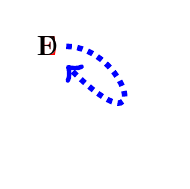
\begin{tikzpicture}[->]
				\Tree [ .\node[red] (e) {E}; [ .C [ .B  [ .A ] ] [ .\node (d) {D}; ] ] [ .\node (f) {F}; [ .G ] ] ]
				\draw[dotted,blue,->, line width=2pt] (f)..controls +(east:1) and +(south east:2) .. (d);
			\end{tikzpicture}
		\column{.25\textwidth}\centering
			\begin{tikzpicture}[->]
				\Tree [ .C [ .B  [ .A ] ] [ .D [ .F [ .G ] ] ] ]
			\end{tikzpicture}
		\pause
		\column{.25\textwidth}\centering
			\vline
			
\begin{tikzpicture}[->]
				\Tree [ .\node[red] (e) {E}; [ .\node (c) {C}; [ .B  [ .A ] ] [ .D ] ] [ .\node (f) {F}; [ .G ] ] ]
				\draw[dotted,blue,->, line width=2pt] (c)..controls +(east:1) and +(west:1) .. (f);
			\end{tikzpicture}
		\column{.25\textwidth}\centering
			\begin{tikzpicture}[->]
				\Tree [ .F [ .C [ .B  [ .A ] ] [ .D ] ] [ .G ] ]
			\end{tikzpicture}
	\end{columns}
\end{frame}

\begin{frame}[label=notas]
	\framesubtitle{Operação Remover}

	\alt<1-4>{Desvantagens}{(Des)Vantagens} da remoção por fusão? \pause
	\begin{columns}[T]
		\column{.25\textwidth}\centering
		\begin{tikzpicture}[->]
			\Tree [ .\node[red] (r) {15};
					[ .10 [ .5 ] [ .11 [ .\node (a) {12}; ] ] ]
					[ .30 [ .20 ] [ .40 ] ]
				 ]
			\node<2->[draw, dashed,line width=2pt, blue, fit=(a)] {};
		\end{tikzpicture}
		\pause
		\column{.25\textwidth}\centering
		\begin{tikzpicture}[->]
			\Tree [ .10 [ .5 ] [ .11 [ .12 [ .30 [ .20 ] [ .40 ] ] ] ] ]
		\end{tikzpicture}\hfill\vline
		\pause
		\column{.25\textwidth}\centering
		\begin{tikzpicture}[->]
			\Tree [ .\node[red] (r) {15};
					[ .\node (a) {10}; [ .5 [ .4 ] [ .7 ] ] ]
					[ .30 [ .20 ] [ .40 ] ]
				 ]
			\node<4->[draw, dashed,line width=2pt, blue, fit=(a)] {};
		\end{tikzpicture}
		\pause
		\column{.25\textwidth}\centering
		\begin{tikzpicture}[->]
			\Tree [ .10 [ .5 [ .4 ] [ .7 ] ] [ .30 [ .20 ] [ .40 ] ] ]
		\end{tikzpicture}
	\end{columns}
	\pause\vfill
	\begin{columns}[T]
		\column{.5\textwidth}\centering
			A altura \textcolor{redUnB}{aumenta}.
		\column{.5\textwidth}\centering
			A altura \textcolor{greenUnB}{diminui}.
	\end{columns}
\end{frame}

\begin{frame}[label=notas]
	\framesubtitle{Operação Remover}

	(Des)Vantagens da remoção por fusão?\pause
	\begin{columns}[T]
		\column{.35\textwidth}\centering
		\begin{tikzpicture}[->]
			\Tree [ .\node (n2) {2};
					[ .\node (n1) {1}; ]
					[ .\node[red] (r) {5};
						[ .\node (n3) {3}; \edge[white]; \node {}; [ .\node (n4) {4}; ] ]
						[ .\node (n9) {9};
							[ .\node (n7) {7};
								[ .\node (n6) {6}; ]
								[ .\node (n8) {8}; ] ] \edge[white]; \node {}; ] ] ]
			\node<3->[subtree, blueUnB, fit=(n1) (n2)] {};
			\node<3->[subtree, gray, fit=(n3) (n4)] {};
			\node<3->[subtree, greenUnB, fit=(n6) (n7) (n8) (n9)] {};
		\end{tikzpicture}
		\pause
		\column{.3\textwidth}
		\ \\\ \\
		- 3 árvores!\\\ \\\pause
		- rotação da de raiz 9
		\column{.35\textwidth}\centering
		\begin{tikzpicture}[->]
			\Tree [ .2
					[ .1 ]
					[ .6
						[ .3 \edge[white]; \node {}; [ .4 ] ]
						[ .9
							[ .7 \edge[white]; \node {};  .8 ]
							\edge[white]; \node[draw=white] {}; ] ] ]
		\end{tikzpicture}
	\end{columns}
\end{frame}

\begin{frame}[label=notas]
	\framesubtitle{Operação Remover}

	Remoção de nó com 2 filhos \pause - \alert<2>{Cópia}:
	o nó não é retirado, mas tem seu conteúdo alterado\pause
		\begin{itemize}
			\item é substituído pelo elemento antecessor \uncover<4->{ou sucessor.}
				\begin{itemize}
					\item Para encontrar o nó antecessor, desce para a subárvore da esquerda, e caminha até o final da subárvore da direita.
					\uncover<4->{\item Para encontrar o nó sucessor, desce para a subárvore da direita do nó a ser retirado, e caminha até o final da subárvore esquerda.}
				\end{itemize}
			\item o substituto é removido conforme seus filhos
		\end{itemize}
	%\Large
	\begin{columns}[T]
		\column{.25\textwidth}\centering
			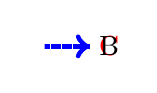
\begin{tikzpicture}[->]
				\Tree [ .\node[red] (c) {C}; [ .A [ .\node (b) {B}; ] ] [ .E [ .D ] [ .F ] ] ]
				\draw[dotted,blue,->, line width=2pt] (b)..controls +(west:1) and +(west:1) .. (c);
			\end{tikzpicture}
		\column{.2\textwidth}\centering
			\begin{tikzpicture}[->]
				\Tree [ .B [ .A ] [ .E [ .D ] [ .F ] ] ]
			\end{tikzpicture}
		\pause
		\column{.35\textwidth}\centering
			\vline\hfill
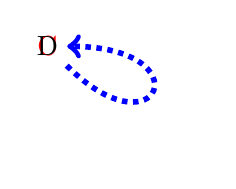
\begin{tikzpicture}[->]
				\Tree [ .\node[red] (c) {C}; [ .A [ .B ] ] [ .E [ .\node (d) {D}; ] [ .F ] ] ]
				\draw[dotted,blue,->, line width=2pt] (d)..controls +(south east:2) and +(east:2) .. (c);
			\end{tikzpicture}
		\column{.2\textwidth}\centering
			\begin{tikzpicture}[->]
				\Tree [ .D [ .A [ .B ] ] [ .E [ .F ] ] ]
			\end{tikzpicture}
	\end{columns}
\end{frame}

\begin{frame}[label=notas]
	\framesubtitle{Operação Remover}

	(Des)Vantagens da remoção por cópia?\pause
	\begin{itemize}
		\item Se aplicado várias vezes (inserção/remoção) a árvore terá um dos
		lados maior que o outro: ou seja a árvore ficará desbalanceada.
		\item O algoritmo pode ser alterado para se tornar simétrico.
			\subitem{Apesar de melhorias significativas, a árvore ainda se tornará
			desbalanceada após muitas operações.}
	\end{itemize}
\end{frame}

%\begin{frame}[fragile,label=notas]
%	\framesubtitle{Travessia/Percurso/Transversalização}
%
%	Travessia: \pause percorrer cada elemento uma única vez.\pause
%
%	\begin{center}
%		\begin{minipage}{.75\textwidth}
%		\begin{lstlisting}[morekeywords={travessia_em_arvore,estado_inicial,vazia,retira_um,objetivo,expande}]
%			travessia_em_arvore(problema)
%			a_visitar:= estado_inicial(problema)
%				enquanto(verdadeiro)
%					se(a_visitar= emptyset) retorna FALHA
%					folha:= retira_um(a_visitar)
%					se(folha = objetivo(problema)) retorna SUCESSO
%					a_visitar += expande(folha)
%		\end{lstlisting}
%		\end{minipage}
%		\end{center}
%\end{frame}
%
%	comparativo buscas
%function TREE-SEARCH(problem) returns a solution, or failure
%	initialize the frontier using the initial state of problem
%	loop do
%		if the frontier is empty then return failure
%		choose a leaf node and remove it from the frontier
%		if the node contains a goal state then return the corresponding solution
%		expand the chosen node, adding the resulting nodes to the frontier
\begin{frame}[label=notas]
	\framesubtitle{Travessia}

		\begin{center}
			\large
			\begin{tikzpicture}[->]
				\unbalancedbinarytree
			\end{tikzpicture}
		\end{center}

	Travessia: \pause percorrer cada elemento uma única vez.\pause
	\begin{itemize}[<+->]
		\item pré-ordem (50, 17, 9, 14, 12, 23, 19, 76, 54, 72, 67) %(os filhos de um nó são processados após o nó)
		\item pós-ordem (12, 14, 9, 19, 23, 17, 67, 72, 54, 76, 50)%(os filhos são processados antes do nó)
		\item em-ordem (9, 12, 14, 17, 19, 23, 50, 54, 67, 72, 76)%(árvores binárias)
		\item ordem de nível (50, 17, 76, 9, 23, 54, 14, 19, 72, 12, 67)
	\end{itemize}
\end{frame}

% \begin{frame}[fragile,label=notas]
% 	\framesubtitle{Travessia Pré-ordem}

% 	Os filhos de um nó são processados após o nó
% 	\begin{columns}[T]
% 		\column{.55\textwidth}\centering\hrule
% 			\begin{lstlisting}
% 				void pre_ordem(bt_node_t *node) {
% 				  if(!node) return;

% 				  processa(node->dado);
% 				  pre_ordem(node->esq);
% 				  pre_ordem(node->dir);
% 				}
% 			\end{lstlisting}
% 		\column{.45\textwidth}\centering
% 			\begin{tikzpicture}[->]
% 				\large
% 				\unbalancedbinarytree
% 			\end{tikzpicture}
% 	\end{columns}
% 	\vfill
% 	\Large 50, 17, 9, 14, 12, 23, 19, 76, 54, 72, 67
% \end{frame}

% \begin{frame}[fragile,label=notas]
% 	\framesubtitle{Travessia Pós-ordem}

% 	Os filhos são processados antes do nó
% 	\begin{columns}[T]
% 		\column{.55\textwidth}\centering
% 			\begin{lstlisting}
% 				void pos_ordem(bt_node_t *node) {
% 				  if(!node) return;

% 				  pos_ordem(node->esq);
% 				  pos_ordem(node->dir);
% 				  processa(node->dado);
% 				}
% 			\end{lstlisting}
% 		\column{.45\textwidth}\centering
% 			\begin{tikzpicture}[->]
% 				\large
% 				\unbalancedbinarytree
% 			\end{tikzpicture}
% 	\end{columns}
% 	\vfill
% 	\Large 12, 14, 9, 19, 23, 17, 67, 72, 54, 76, 50
% \end{frame}

% \begin{frame}[fragile,label=notas]
% 	\framesubtitle{Travessia Em-ordem}

% 	O nó é processado entre os filhos
% 	\begin{columns}[T]
% 		\column{.55\textwidth}\centering
% 			\begin{lstlisting}
% 				void em_ordem(bt_node_t *node) {
% 				  if(!node) return;

% 				  em_ordem(node->esq);
% 				  processa(node->dado);
% 				  em_ordem(node->dir);
% 				}
% 			\end{lstlisting}
% 		\column{.45\textwidth}\centering
% 			\begin{tikzpicture}[->]
% 				\large
% 				\unbalancedbinarytree
% 			\end{tikzpicture}
% 	\end{columns}
% 	\vfill
% 	\Large 9, 12, 14, 17, 19, 23, 50, 54, 67, 72, 76
% \end{frame}

% \begin{frame}[fragile,label=notas]
% 	\framesubtitle{Travessia Ordem de Nível}

% 	Cada nó é processado junto aos do seu nível
% 	\begin{columns}[T]
% 		\column{.55\textwidth}\centering
% 			\begin{lstlisting}
% 				void ordem_de_nivel(bt_node_t *node) {
% 				  if(!node) return;
% 				  fila_t *fila = nova_fila();
% 				  node_t *ptr;
% 				  insere_na_fila(fila, node);
% 				  while(!vazia(fila)) {
% 				    ptr = retira_da_fila(fila);
% 				    processa(ptr->dado);
% 				    if(ptr->esq)
% 				      insere_na_fila(fila, ptr->esq);
% 				    if(ptr->dir)
% 				      insere_na_fila(fila, ptr->dir);
% 				  }
% 				}
% 			\end{lstlisting}
% 		\column{.45\textwidth}\centering
% 			\begin{tikzpicture}[->]
% 				\large
% 				\unbalancedbinarytree
% 			\end{tikzpicture}
% 	\end{columns}
% 	\Large 50, 17, 76, 9, 23, 54, 14, 19, 72, 12, 67
% \end{frame}

\begin{frame}[label=notas]
	\frametitle{Árvore Binária}
	\framesubtitle{Expressões contendo operadores binários}

	\begin{center}
		\begin{tikzpicture}[->, level distance=15mm, every node/.style={circle, draw}]%[level distance=10mm,]%[level/.style={sibling distance=25mm}]
			\Large \Tree [./
					[ .+
						[ .A ]
						[ .*
							[ .B ] [ .C ] ] ]
					[ .*
						[ .+
							[ .A ] [ .B ] ]
						[ .C ] ]
				]
		\end{tikzpicture}
	\end{center}
	\begin{itemize}
		\item Pós-ordem:  \pause $ABC*+AB+C*/$ \pause $\leftarrow$ forma \emph{pós-fixada}
		\item Pré-ordem: \pause $/+A*BC*+ABC$ $\leftarrow$ forma \emph{pré-fixada}
		\item Em ordem: \pause $A+B*C/A+B*C$ $\leftarrow$ forma \emph{infixada}
	\end{itemize}
\end{frame}

\begin{frame}[fragile,label=notas]
	\framesubtitle{Busca}

	\pause
	Os elementos da árvore binária estão ordenados, a busca na árvore faz uso de um algoritmo simples:
	\pause
	\subitem{Compare o elemento com a raiz:
		\begin{enumerate}
			\item se for igual, pare a  busca; se for menor, busque na subárvore da esquerda
			\item se for maior, busque na para a subárvore da direita
		\end{enumerate}
	}
\end{frame}

\begin{frame}[fragile,label=notas]
	\framesubtitle{Operação Buscar}

	\pause
	\begin{center}
		\begin{minipage}{.72\textwidth}
			\begin{lstlisting}
				bt_node_t *busca_nos(bt_node_t *node, dado_t dado) {
				  if(!node) return NULL;

				  if(dado < node->dado)
				    return busca_nos(node->esq, dado);
				  if(dado > node->dado)
				    return busca_nos(node->dir, dado);

				  return node;
				}
			\end{lstlisting}
		\end{minipage}
	\end{center}
\end{frame}

\begin{frame}[label=notas]
	\framesubtitle{Procurando um número}

	\begin{center}
		\begin{tikzpicture}[->, level distance=18mm]
			\Huge
			\balancedbinarytree
		\end{tikzpicture}
	\end{center}
\end{frame}

\begin{frame}[label=notas]
	\framesubtitle{Procurando uma palavra}

	\begin{center}
		\Large
		\begin{tikzpicture}[->, level distance=18mm]
			\Tree [ .Itaipava
					[ .Bohemia
						[ .Antártica ]
						[ .Brahma ] ]
					[ .Original
						\edge[white]; [ .\node[circle, draw=white](n1){}; ]
						[ .Terezópolis
							[ .Skol ]
							\edge[white]; [ .\node[circle, draw=white](n1){}; ] ] ] ]
		\end{tikzpicture}
	\end{center}
\end{frame}

\begin{frame}[label=notas]
	Eficiência da árvore como estrutura de busca \alert<1>{depende da disposição de seus elementos}! \pause
	\\ Qual o pior caso?
	\begin{columns}[T]
		\column{.3\textwidth}{\centering
			\begin{tikzpicture}[->]
				\Tree [ .K [ .B \edge[white]; \node {};  [ .D ] ] [ .P [ .M ] [ .R ] ] ]
			\end{tikzpicture}}
			\\\pause
			3 comparações
		\column{.3\textwidth}{\centering
			\begin{tikzpicture}[->]
				\Tree [ .B \edge[white]; \node {};
						[ .K [ .D ]
							[ .P [ .M ] [ .R ] ] ] ]
			\end{tikzpicture}}
			\\\pause
			4 comparações
		\column{.3\textwidth}\centering
			\begin{tikzpicture}[->]
			                 	\Tree [ .B \edge[white]; \node {};
			                 		[ .D \edge[white]; \node {};
			                 			[ .K \edge[white]; \node {};
			                 				[ .P \edge[white]; \node {};
			                 					[ .M \edge[white]; \node {};
			                 						[ .R ] ] ] ] ] ]
			\end{tikzpicture}
	\end{columns}
	\vspace{-2\baselineskip}\pause
	\hfill árvore degenerada em lista! $\Leftarrow$ 6 comparações\hspace{2cm}
\end{frame}

\subsection*{Árvore Binária Balanceada}
\begin{frame}[label=notas]
	\alert<1>{Árvore binária balanceada}: para cada nó, as alturas de suas subárvores diferem de, no máximo, 1.
		\subitem{É  a árvore com menor altura para o seu número de nós.}
	\begin{columns}[T]
		\column{.45\textwidth}\centering
			\begin{tikzpicture}[->, sibling distance=5mm]
				\Tree [ .\node (d) {D};
							[ .\node (c) {C};
								[ .\node (b) {B};
									[ .\node (a) {A}; ]
									\edge[white]; \node {}; ]
								\edge[white]; \node (c1) {}; ]
							[ .\node (e) {E};
								\edge[white]; \node {};
								[ .F \edge[white]; \node {};
								[ .\node (g) {G}; ] ] ] ]
				\node<2-3 | handout:0>[thickcircle, orange, fit=(d)] {};
				\node<3 | handout:0>[subtree, greenUnB!50, fit=(a) (c)] {};
				\node<3 | handout:0>[subtree, blueUnB!50, fit=(e) (g)] {};

				\node<4-5>[thickcircle, orange, fit=(c)] {};
				\node<5>[subtree, greenUnB!50, fit=(a) (b)] {};
				\node[subtree, blueUnB!50, fit=(c1)] {};
			\end{tikzpicture}
		\column{.45\textwidth}\centering
			\uncover<6->{
			\begin{tikzpicture}[->, sibling distance=5mm]
				\Tree [ .\node (b) {B};
							[ .\node (a) {A}; ]
							[ .\node (d) {D};
								[ .\node (c) {C}; ]
								[ .F 	[ .E ]
									[ .H
										[ .G ]
										[ .\node (i) {I}; ]
							] ] ] ]
				\node<7->[thickcircle, orange, fit=(b)] {};
				\node<8>[subtree, greenUnB!50, fit=(a)] {};
				\node<8>[subtree, blueUnB!50, fit=(c) (d) (i)] {}; %erro de underfill... ???
			\end{tikzpicture}}
	\end{columns}
\end{frame}

\begin{frame}[fragile,label=notas]
	\begin{columns}[T]
		\column{.5\textwidth}\centering
			\begin{tikzpicture}[->, sibling distance=5mm]
				\Tree [ .\node (d) {D};
							[ .\node (b) {B};
								[ .\node (a) {A}; ]
								[ .\node (c) {C}; ] ]
							[ .\node (e) {E};
								\edge[white]; \node (e1) {};
								[ .\node (g) {G};
									[ .\node (f) {F}; ]
									[ .\node (h) {H};  ] ] ] ]
				\node<2-3 | handout:0>[thickcircle, orange, fit=(d)] {};
				\node<3 | handout:0>[subtree, greenUnB!50, fit=(a) (b) (c)] {};
				\node<3 | handout:0>[subtree, blueUnB!50, fit=(e) (f) (h)] {};

				\node<4-5 | handout:0>[thickcircle, orange, fit=(b)] {};
				\node<5 | handout:0>[subtree, greenUnB!50, fit=(a)] {};
				\node<5 | handout:0>[subtree, blueUnB!50, fit=(c)] {};

				\node<6->[thickcircle, orange, fit=(e)] {};
				\node<7->[subtree, greenUnB!50, fit=(e1)] {};
				\node<7->[subtree, blueUnB!50, fit=(f) (g) (h)] {};
			\end{tikzpicture}
		\column{.5\textwidth}\centering
			\begin{lstlisting}[morekeywords={abs}]
				char balanceada(node_t *raiz){
				    if (vazia(raiz))
				        return 1; //verdadeiro
				    if(!balanceada(raiz->esq))
				        return 0; // falso
				    if(!balanceada(raiz->dir))
				        return 0; // falso
				    if(abs(altura(raiz->esq) - altura(raiz->dir)) > 1)
				        return 0; // falso
				    return 1; // verdadeiro
				}
			\end{lstlisting}
	\end{columns}
\end{frame}

\begin{frame}[label=notas]
	O objetivo desta árvore é estruturar os dados de forma flexível, permitindo pesquisa binária \uncover<2->{$\rightarrow$ custo de tempo para pesquisa: $O(log_2(n))$}
	\begin{columns}
		\column{.4\textwidth}\centering
			\begin{tikzpicture}[->]
				\balancedbinarytree
			\end{tikzpicture}
		\column{.6\textwidth}\centering
			 \uncover<2->{
			 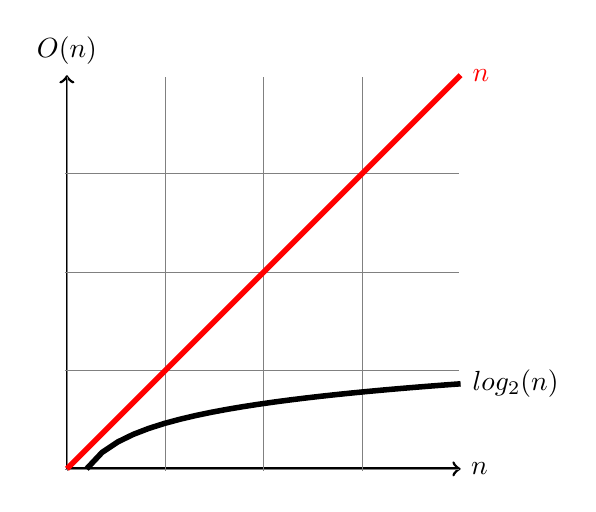
\begin{tikzpicture}[line width=2pt, scale=.25]
				\draw[->,line width=1pt] (0,0) -- (20,0) node[right] {$n$};
				\draw[->,line width=1pt] (0,0) -- (0,20) node[above] {$O(n)$};
				\draw[very thin,color=gray] (-0.1,-0.1) grid[step=5] (19.9,19.9);
				\draw[color=red, domain=0:20] plot (\x,\x) node[right] {$n$};
				\draw[domain=1:20] plot (\x, {log2(\x)}) node[right] {$log_2(n)$};
			\end{tikzpicture}}
	\end{columns}
\end{frame}

\begin{frame}[label=notas]
	A maioria das operações depende diretamente da altura da árvore (daí o desejo de se ter a menor possível).
	\begin{center}
		\large
		\begin{tabular}{| c | c | c |}
			\hline
			\textbf{Altura} & \textbf{Nós em um nível} & \textbf{Total de nós} \\\hline
			1 & 1 & 1 \\\hline
			2 & 2 & 3 \\\hline
			3 & 4 & 7 \\\hline
			4 & 8 & 15 \\\hline
			11 & 1024 & 2047 \\\hline
			14 & 8192 & 16383 \\\hline
			$h$ & $2^{h-1}$ & $2^h-1$ \\\hline
		\end{tabular}
	\end{center}
	\begin{itemize}
		\item $h$ é o número \alert{máximo} de testes a serem feitos \pause $\rightarrow$ custo no \emph{pior caso}.
		\item Como o número máximo de nós possíveis é $n \le 2^h-1$,
		\begin{center}
			$h\ge\lceil\log_2(n+1)\rceil\ge \lfloor\log_2 n\rfloor$
		\end{center}
	\end{itemize}
\end{frame}

\begin{frame}[label=notas]
	Algoritmos para Balanceamento
	\begin{itemize}
		\item Estático: destruir a estrutura da árvore e reconstruí-la balanceada
			\begin{itemize}
				\item Vetor
				\item DSW (Day/Stout/Warren)
			\end{itemize}
		\item Dinâmico: balanceamento junto as operações
			\begin{itemize}
				\item AVL (Adelson-Velskii e E.M. Landis)
				\item Rubro-negra
			\end{itemize}
	\end{itemize}
\end{frame}

\begin{frame}[label=notas]
	\framesubtitle{Balanceamento Estático (Vetor)}

	Vetor: os dados da árvore são armazenados em um vetor (ou lista), ordenados,
	e outra árvore é construída a partir deste. \\\vfill
	\begin{columns}
		\large
		\column{.25\textwidth}\centering
			\begin{tikzpicture}[->]
				\Tree [ .B \edge[white]; \node {};
						[ .K [ .D ]
							[ .P [ .M ] [ .R ] ] ] ]
			\end{tikzpicture}
		\column{.5\textwidth}\centering
			{\normalsize Vetor ordenado}
			\begin{tabular}{|*{6}{ c |}}
				\hline B & D & K & M & P & R\\\hline
			\end{tabular}\\ \vfill
			\pause
			\begin{tabular}{|*{6}{ c |}}
				\multicolumn{1}{ c }{} & \multicolumn{3}{ c }{Raiz} & \multicolumn{2}{ c }{}\\\cline{3-3}
				\multicolumn{2}{ c }{} & \multicolumn{1}{| c |}{\cellcolor{redUnB!50}K} & \multicolumn{3}{ c }{}\\\hline
				\cellcolor{greenUnB!50}B & \cellcolor{greenUnB!50}D &  & \cellcolor{blueUnB!50}M & \cellcolor{blueUnB!50}P & \cellcolor{blueUnB!50}R\\\cline{1-2}\cline{4-6}
				\multicolumn{2}{ c }{$S_E$} &  \multicolumn{1}{ c }{} & \multicolumn{3}{ c }{$S_D$}
			\end{tabular}\\ \vfill
			{\normalsize \pause
			\begin{tabular}{*{6}{ c }}
				\cline{3-3}
				& & \multicolumn{1}{| c |}{K} & & \\ \cline{1-1}\cline{3-3}\cline{5-5}
				 \multicolumn{1}{| c |}{\cellcolor{redUnB!50}B} & &  & &  \multicolumn{1}{| c |}{\cellcolor{redUnB!50}P} & \\\cline{1-2}\cline{4-6}
				& \multicolumn{1}{| c |}{\cellcolor{blueUnB!50}D} & & \multicolumn{1}{| c |}{\cellcolor{greenUnB!50}M} & & \multicolumn{1}{| c |}{\cellcolor{blueUnB!50}R} \\\cline{2-2}\cline{4-4}\cline{6-6}
			\end{tabular}
			}
		\pause
		\column{.2\textwidth}\centering
			\begin{tikzpicture}[->]
				\Tree [ .K [ .B \edge[white]; \node {};  D ]
						[ .P [ .M ] [ .R ] ] ]
			\end{tikzpicture}
	\end{columns}
\end{frame}